\chapter{Sprint 3 : Validation et traçabilité}
\newpage
\section{Introduction}


Le cinquième chapitre présente les réalisations du Sprint 3. Nous abordons les fonctionnalités de validation financière, le traitement des anomalies, la gestion des commentaires ainsi que la traçabilité des actions à travers le journal des opérations.


\section{Backlog du Sprint}

\renewcommand{\arraystretch}{1.25}

\begin{table}[H]
	\centering
	\footnotesize
	
	\begin{tabularx}{\textwidth}{|c|p{3.6cm}|c|X|c|}
		\hline
		
		\rowcolor{blue!20}
		\textbf{ID} &
		\textbf{User Story} &
		\textbf{ID-US} &
		\textbf{Tâche} &
		\textbf{Estimation}
		\\ \hline
		
		\multirow{5}{*}{3.1}
		& \multirow{5}{3.6cm}{
			En tant que responsable financier, je veux gérer les validations financières afin de contrôler les factures.
		}
		& 3.1.1 & Conception UML des validations financières. & \multirow{5}{*}{3 jours}
		\\ \cline{3-4}
		
		& & 3.1.2 & Développement de l’interface de validation.
		& \\ \cline{3-4}
		
		& & 3.1.3 & Implémentation des actions approuver/rejeter.
		& \\ \cline{3-4}
		
		& & 3.1.4 & Ajout du système de commentaires obligatoires.
		& \\ \cline{3-4}
		
		& & 3.1.5 & Tests et validation.
		& \\ \hline
		
		\multirow{4}{*}{3.2}
		& \multirow{4}{3.6cm}{
			En tant que responsable financier, je veux voir et modifier les données d’une facture afin de corriger les erreurs détectées.
		}
		& 3.2.1 & Conception UML de consultation et modification. & \multirow{4}{*}{2 jours}
		\\ \cline{3-4}
		
		& & 3.2.2 & Développement de l’interface voir facture.
		& \\ \cline{3-4}
		
		& & 3.2.3 & Développement de l’interface de modification.
		& \\ \cline{3-4}
		
		& & 3.2.4 & Tests et validation.
		& \\ \hline
		
		\multirow{4}{*}{3.3}
		& \multirow{4}{3.6cm}{
			En tant que responsable financier, je veux consulter le tableau de bord financier afin de suivre les opérations financières.
		}
		& 3.3.1 & Conception du tableau de bord financier. & \multirow{4}{*}{2 jours}
		\\ \cline{3-4}
		
		& & 3.3.2 & Développement des graphiques et indicateurs.
		& \\ \cline{3-4}
		
		& & 3.3.3 & Intégration des statistiques dynamiques.
		& \\ \cline{3-4}
		
		& & 3.3.4 & Tests et validation.
		& \\ \hline
		
		\multirow{4}{*}{3.4}
		& \multirow{4}{3.6cm}{
			En tant qu’administrateur, je veux consulter le journal des actions afin d’assurer la traçabilité des opérations.
		}
		& 3.4.1 & Conception UML du journal des actions. & \multirow{4}{*}{1 jour}
		\\ \cline{3-4}
		
		& & 3.4.2 & Développement de l’interface du journal.
		& \\ \cline{3-4}
		
		& & 3.4.3 & Implémentation du stockage des actions.
		& \\ \cline{3-4}
		
		& & 3.4.4 & Tests et validation.
		& \\ \hline
		
	\end{tabularx}
	
	\caption{Backlog détaillé du Sprint 3}
	\label{tab:backlog_sprint3}
	
\end{table}

\FloatBarrier



\section{Analyse}

\subsection{Analyse fonctionnelle}

\subsubsection{Diagramme de cas d’utilisation}

Le diagramme de cas d’utilisation montre les fonctions du troisième sprint. Le diagramme montre le responsable financier qui valide les factures et qui consulte le tableau de bord financier. Le diagramme montre aussi l’administrateur qui consulte le journal des actions.

\begin{figure}[H]
	\centering
	
\includegraphics[width=0.9\textwidth]{usecase_sprint3.jpg}
	\caption{Diagramme de cas d’utilisation du Sprint 3}
	\label{fig:usecase_sprint3}
\end{figure}

\FloatBarrier

\subsubsection{Description textuelle des cas d’utilisation}

\subsubsection*{Cas d’utilisation : Gérer les validations financières}

\begin{table}[H]
	\centering
	\renewcommand{\arraystretch}{1.5}
	\small
	\begin{tabularx}{\textwidth}{|p{4.5cm}|X|}
		\hline
		\rowcolor{blue!20}
		\textbf{Nom du cas d’utilisation} & Gérer les validations financières \\ \hline
		
		\textbf{Description brève} & Le responsable financier consulte les détails d’une facture, peut voir le document original, modifier les données si nécessaire, puis approuver ou rejeter la facture avec un commentaire obligatoire. \\ \hline
		
		\textbf{Acteurs primaires} & Responsable financier \\ \hline
		
		\textbf{Acteurs secondaires} & Aucun \\ \hline
		
		\textbf{Pré-condition} & Le responsable financier doit être authentifié. \\ \hline
		
		\textbf{Scénario nominal} &
		1- Le responsable financier ouvre l’interface des validations. \newline
		2- Le système affiche les factures en attente. \newline
		3- Le responsable financier clique sur le bouton « Détails ». \newline
		4- Le système affiche les informations détaillées de la facture. \newline
		5- Si le responsable financier choisit « Voir facture » : \newline
		\hspace*{0.5cm}5.1- Le système affiche le document original de la facture. \newline
		6- Si le responsable financier choisit « Modifier » : \newline
		\hspace*{0.5cm}6.1- Le système active le mode modification. \newline
		\hspace*{0.5cm}6.2- Le responsable financier modifie les données nécessaires. \newline
		\hspace*{0.5cm}6.3- Le système vérifie et enregistre les modifications. \newline
		7- Si le responsable financier choisit « Approuver » : \newline
		\hspace*{0.5cm}7.1- Le responsable financier saisit un commentaire obligatoire. \newline
		\hspace*{0.5cm}7.2- Le système valide la facture. \newline
		\hspace*{0.5cm}7.3- Le système enregistre l’action dans le journal. \newline
		8- Si le responsable financier choisit « Rejeter » : \newline
		\hspace*{0.5cm}8.1- Le responsable financier saisit un commentaire obligatoire. \newline
		\hspace*{0.5cm}8.2- Le système rejette la facture. \newline
		\hspace*{0.5cm}8.3- Le système enregistre l’action dans le journal. \\ \hline
		
		\textbf{Post-condition} & La facture est modifiée si nécessaire, puis validée ou rejetée avec une action enregistrée dans le journal. \\ \hline
		
		\textbf{Scénarios alternatifs} &
		1- Commentaire non saisi. \newline
		1.1- Le système bloque l’approbation ou le rejet. \newline
		2- Données modifiées invalides. \newline
		2.1- Le système refuse l’enregistrement. \newline
		3- Facture introuvable. \newline
		3.1- Le système annule l’opération. \\ \hline
		
	\end{tabularx}
	\caption{Description textuelle du cas d’utilisation « Gérer les validations financières »}
	\label{tab:validation_financiere}
\end{table}

\FloatBarrier

\subsubsection*{Cas d’utilisation : Consulter le journal des actions}

\begin{table}[H]
	\centering
	\renewcommand{\arraystretch}{1.35}
	\rowcolors{2}{gray!10}{white}
	\begin{tabularx}{\textwidth}{|p{3.8cm}|X|}
		\hline
		\rowcolor{blue!20}
		\textbf{Use Case} & Consulter le journal des actions \\ \hline
		
		\textbf{Acteur} & Administrateur \\ \hline
		
		\textbf{Description} & Permet à l’administrateur de consulter l’historique des actions effectuées dans le système afin d’assurer la traçabilité des opérations. \\ \hline
		
		\textbf{Pré-condition} & L’administrateur est authentifié. \\ \hline
		
		\rowcolor{blue!10}
		\textbf{Scénario nominal} &
		1- L’administrateur ouvre l’interface du journal. \newline
		2- Le système récupère les actions qui ont été enregistrées. \newline
		3- Le système affiche la liste des actions. \newline
		4- L’administrateur regarde les informations affichées. \\ \hline
		
		\textbf{Post-condition} & Le journal des actions est affiché. \\ \hline
		
		\rowcolor{blue!10}
		\textbf{Scénarios alternatifs} &
		1- Aucun historique disponible. \newline
		1.1- Le système affiche un message informatif. \newline
		2- Erreur lors du chargement du journal. \newline
		2.1- Le système affiche un message d’erreur. \\ \hline
		
	\end{tabularx}
	\caption{Description textuelle du cas d’utilisation « Consulter le journal des actions »}
	\label{tab:journal_actions}
\end{table}

\FloatBarrier

\subsection{Analyse dynamique}

\subsubsection{Diagramme de séquence système du cas d’utilisation « Gérer les validations financières »}

Le diagramme de séquence système montre les interactions entre le responsable financier et le système. Le diagramme de séquence système décrit le processus d’approbation ou de rejet d’une facture par le responsable financier.

\begin{figure}[H]
	\centering
	
\includegraphics[width=0.85\textwidth]{seq_system_validation.jpg}
	\caption{Diagramme de séquence système - Gérer les validations financières}
	\label{fig:seq_system_validation}
\end{figure}

\FloatBarrier

\subsubsection{Diagramme de séquence système du cas d’utilisation « Consulter le journal des actions »}

Le diagramme suivant montre les interactions entre l’administrateur et le système. L’administrateur consulte le journal des actions.

\begin{figure}[H]
	\centering
	
\includegraphics[width=0.85\textwidth]{seq_system_journal.jpg}
	\caption{Diagramme de séquence système - Consulter le journal des actions}
	\label{fig:seq_system_journal}
\end{figure}

\FloatBarrier

\section{Conception}
\subsection{Conception statique}

\subsubsection{Diagramme de classes du Sprint 3}

Le diagramme de classes montre les entités manipulées pendant ce sprint. Il indique les factures, les commentaires liés aux décisions et le journal qui assure la traçabilité des actions.

\begin{figure}[H]
	\centering
	
\includegraphics[width=0.85\textwidth]{class_sprint3.jpg}
	\caption{Diagramme de classes du Sprint 3}
	\label{fig:class_sprint3}
\end{figure}

\FloatBarrier
\subsection{Conception dynamique}

\subsubsection{Diagramme de séquence détaillé du cas d’utilisation « Gérer les validations financières »}

Le diagramme suivant montre les interactions entre les différents composants du système lors de l’approbation d’une facture ou du rejet d’une facture. L’ajout d’un commentaire est obligatoire et l’action est enregistrée dans le journal.

\begin{figure}[H]
	\centering
	
\includegraphics[width=0.85\textwidth]{seq_detail_validation.jpg}
	\caption{Diagramme de séquence détaillé - Gérer les validations financières}
	\label{fig:seq_detail_validation}
\end{figure}

\FloatBarrier

\subsubsection{Diagramme de séquence détaillé du cas d’utilisation « Consulter le journal des actions »}

Le diagramme montre les échanges entre l’administrateur, l’interface du journal, le contrôleur et la base de données lors de la consultation de l’historique des actions.

\begin{figure}[H]
	\centering
	
\includegraphics[width=0.85\textwidth]{seq_detail_journal.jpg}
	\caption{Diagramme de séquence détaillé - Consulter le journal des actions}
	\label{fig:seq_detail_journal}
\end{figure}

\FloatBarrier


\section{Implémentation}

\subsection{Dictionnaire de données}

\subsubsection{Table validation}

\renewcommand{\arraystretch}{1.3}

\begin{table}[H]
	\centering
	\footnotesize
	
	\begin{tabularx}{\textwidth}{|p{3cm}|p{2.5cm}|p{3.5cm}|X|}
		\hline
		
		\rowcolor{blue!20}
		\textbf{Nom du champ}
		&
		\textbf{Type}
		&
		\textbf{Contraintes}
		&
		\textbf{Description}
		\\ \hline
		
		id\_validation
		&
		BIGINT
		&
		PRIMARY KEY
		&
		Identifiant unique de la validation.
		\\ \hline
		
		factureId
		&
		BIGINT
		&
		FOREIGN KEY
		&
		Facture concernée par la validation.
		\\ \hline
		
		decision
		&
		VARCHAR
		&
		NOT NULL
		&
		Décision prise sur la facture.
		\\ \hline
		
		commentaire
		&
		TEXT
		&
		NOT NULL
		&
		Commentaire obligatoire ajouté par le responsable.
		\\ \hline
		
		dateValidation
		&
		DATETIME
		&
		NOT NULL
		&
		Date de validation de la facture.
		\\ \hline
		
	\end{tabularx}
	
	\caption{Dictionnaire de données de la table validation}
	\label{tab:validation_table}
	
\end{table}



\subsubsection{Table journal des actions}

\begin{table}[H]
	\centering
	\footnotesize
	
	\begin{tabularx}{\textwidth}{|p{3cm}|p{2.5cm}|p{3.5cm}|X|}
		\hline
		
		\rowcolor{blue!20}
		\textbf{Nom du champ}
		&
		\textbf{Type}
		&
		\textbf{Contraintes}
		&
		\textbf{Description}
		\\ \hline
		
		id\_journal
		&
		BIGINT
		&
		PRIMARY KEY
		&
		Identifiant du journal.
		\\ \hline
		
		utilisateur
		&
		VARCHAR
		&
		NOT NULL
		&
		Nom de l’utilisateur ayant effectué l’action.
		\\ \hline
		
		action
		&
		TEXT
		&
		NOT NULL
		&
		Description de l’action réalisée.
		\\ \hline
		
		dateAction
		&
		DATETIME
		&
		NOT NULL
		&
		Date et heure de l’action.
		\\ \hline
		
	\end{tabularx}
	
	\caption{Dictionnaire de données de la table journal des actions}
	\label{tab:journal_table}
	
\end{table}
\section{Réalisation}

\subsection{Interfaces utilisateur}

\subsubsection{Interface de validation des factures}

Cette interface permet au responsable financier de consulter la liste des factures en attente de décision. Elle affiche les informations principales de chaque facture, telles que le fournisseur, le montant, le score de confiance de l’IA et le statut.

\begin{figure}[H]
	\centering
	
\includegraphics[width=0.85\textwidth]{ui_validation_factures.jpg}
	\caption{Interface de validation des factures}
	\label{fig:ui_validation_factures}
\end{figure}

\FloatBarrier

\subsubsection{Interface des détails de la facture}

Cette interface affiche les informations détaillées de la facture sélectionnée. Elle permet au responsable financier de vérifier les données extraites, de consulter le document original, de modifier les données si nécessaire, puis d’approuver ou de rejeter la facture avec un commentaire obligatoire.

\begin{figure}[H]
	\centering
	
\includegraphics[width=0.85\textwidth]{ui_details_facture.jpg}
	\caption{Interface des détails de la facture}
	\label{fig:ui_details_facture}
\end{figure}

\FloatBarrier

\subsubsection{Interface de modification des données de la facture}

Cette interface permet au responsable financier de corriger les données extraites automatiquement lorsqu’une erreur est détectée.

\begin{figure}[H]
	\centering
	
\includegraphics[width=0.85\textwidth]{ui_modifier_facture.jpg}
	\caption{Interface de modification des données de la facture}
	\label{fig:ui_modifier_facture}
\end{figure}

\FloatBarrier

\subsubsection{Interface du commentaire obligatoire}

Cette interface permet au responsable financier de saisir un commentaire avant toute décision finale.

\begin{figure}[H]
	\centering
	
\includegraphics[width=0.85\textwidth]{ui_commentaire_obligatoire.jpg}
	\caption{Interface du commentaire obligatoire}
	\label{fig:ui_commentaire_obligatoire}
\end{figure}

\FloatBarrier

\subsubsection{Interface du tableau de bord financier}

Cette interface permet au responsable financier de visualiser les indicateurs financiers liés aux factures.

\begin{figure}[H]
	\centering
	
\includegraphics[width=0.65\textwidth]{ui_dashboard_financier.jpg}
	\caption{Interface du tableau de bord financier}
	\label{fig:ui_dashboard_financier}
\end{figure}

\FloatBarrier

\subsubsection{Interface du journal des actions}

Cette interface permet à l’administrateur de consulter l’historique des actions effectuées dans le système.

\begin{figure}[H]
	\centering
	
\includegraphics[width=0.85\textwidth]{ui_journal.jpg}
	\caption{Interface du journal des actions}
	\label{fig:ui_journal}
\end{figure}

\FloatBarrier

\section{Tests Postman}

Cette section présente les tests réalisés avec Postman afin de vérifier les fonctionnalités développées durant le Sprint 3.  
Ces tests concernent principalement la validation financière, le rejet des factures, l’affichage des statistiques et la configuration des seuils de confiance de l’intelligence artificielle.

L’objectif de ces tests est de confirmer que les décisions prises par le responsable financier sont correctement enregistrées et que les actions sont bien tracées dans le système.

\renewcommand{\arraystretch}{1.5}
\newpage
\begin{longtable}{|>{\centering\arraybackslash}m{5cm}|>{\centering\arraybackslash}m{9cm}|}
	\hline
	
	\rowcolor{blue!20}
	\textbf{Description} & \textbf{Capture}
	\\ \hline
	
	Cette requête permet au responsable financier de valider une facture. 
	Elle vérifie que le statut de la facture est mis à jour et que la décision est enregistrée avec un commentaire.
	&
	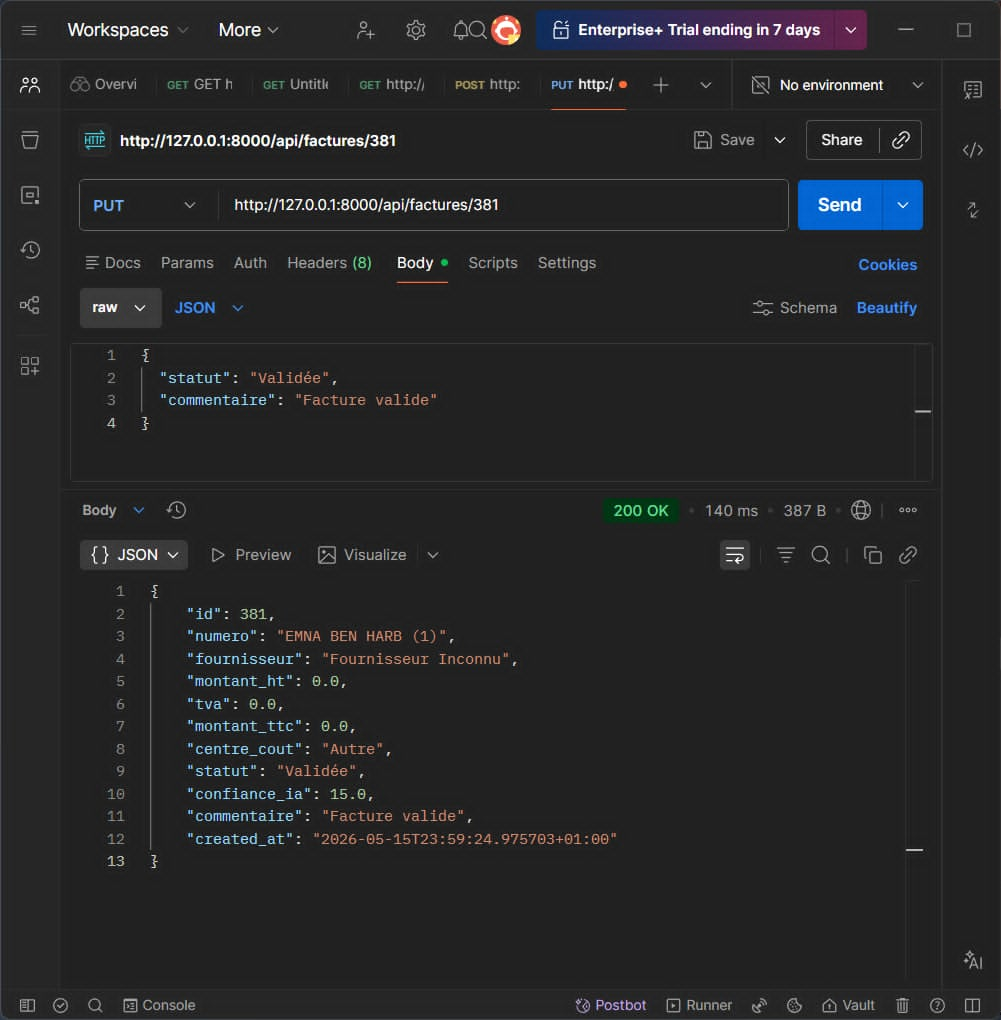
\includegraphics[width=8cm]{figures/postman_validation.jpg}
	\\ \hline
	
	Cette requête permet de rejeter une facture avec un commentaire obligatoire. 
	Elle permet de vérifier que le système refuse ou accepte la décision selon la présence du commentaire justificatif.
	&
	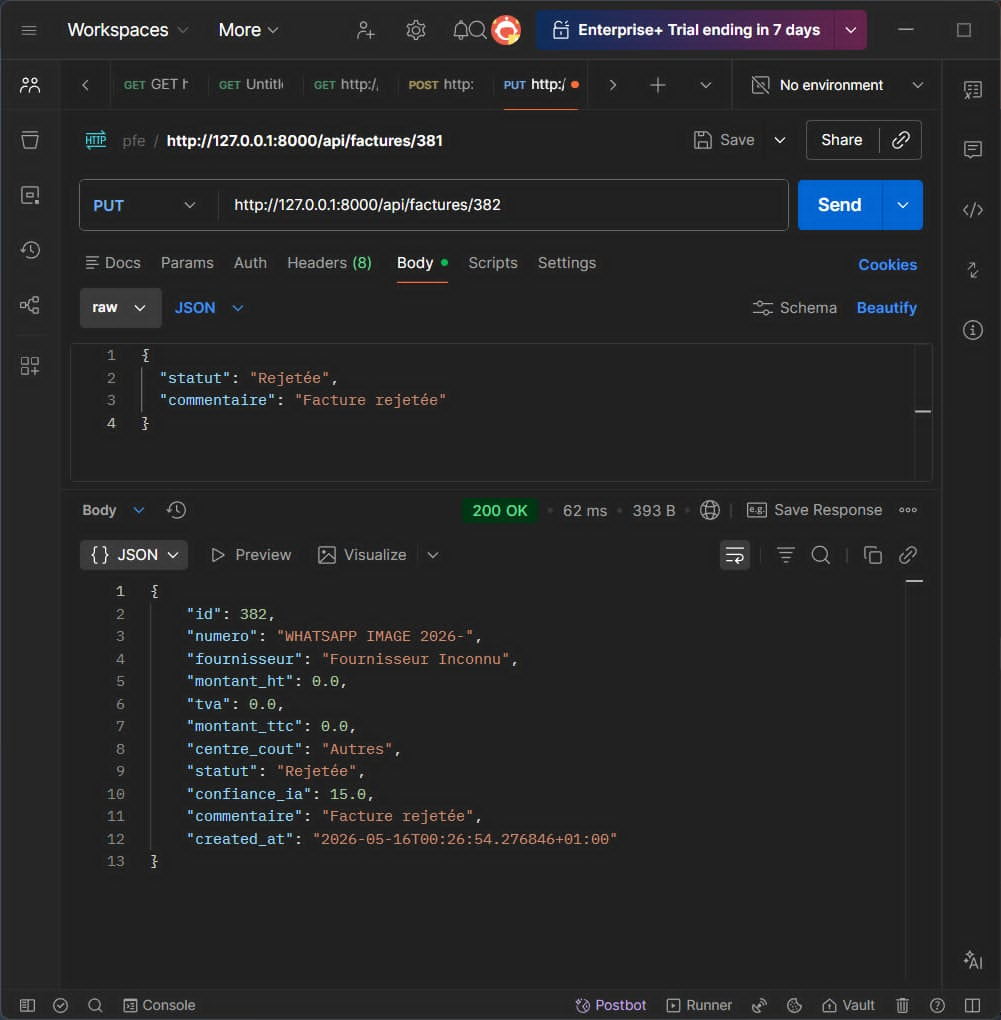
\includegraphics[width=8cm]{figures/postman_rejet.jpg}
	\\ \hline
	
	Cette requête permet d’afficher les statistiques et les indicateurs financiers. 
	Elle vérifie le bon fonctionnement du tableau de bord financier et la récupération des données nécessaires.
	&
	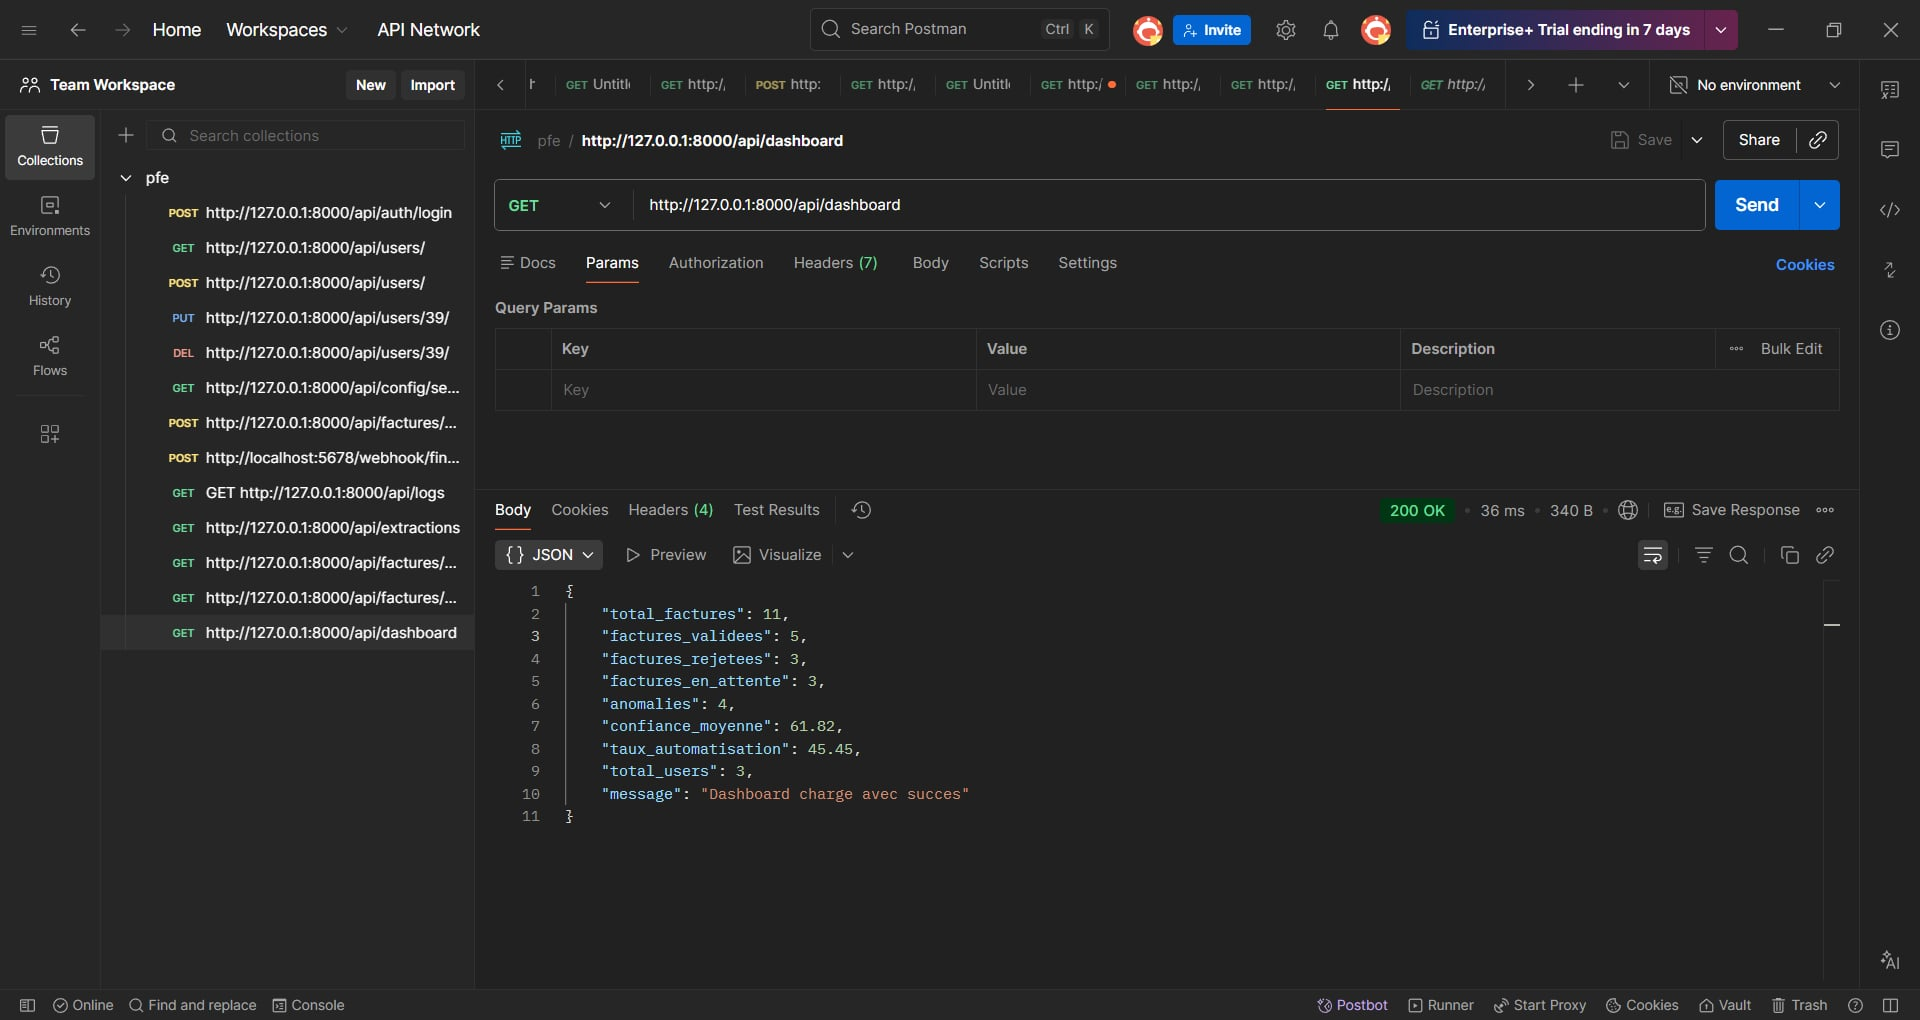
\includegraphics[width=8cm]{figures/postman_dashboard.jpg}
	\\ \hline
	
	Cette requête permet de modifier les seuils de confiance de l’intelligence artificielle. 
	Elle permet à l’administrateur d’ajuster les paramètres utilisés pour proposer automatiquement le statut d’une facture.
	&
	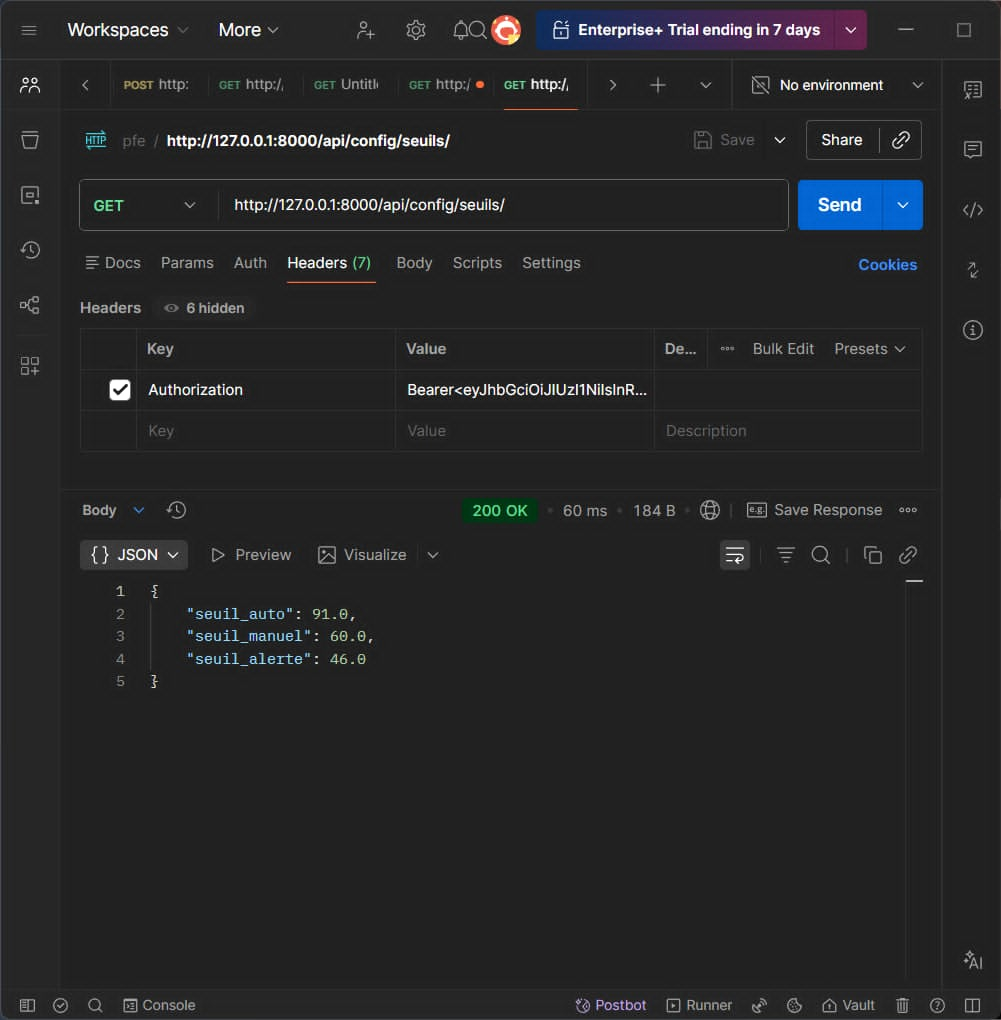
\includegraphics[width=8cm]{figures/postman_config_ia.jpg}
	\\ \hline
	
	\caption{Tests Postman du Sprint 3}
\end{longtable}
\vspace{0.3cm}
\subsection{Revue de Sprint}

La revue du Sprint 3 a permis de présenter les fonctionnalités réalisées concernant la validation financière des factures, la gestion des commentaires obligatoires ainsi que la traçabilité des actions à travers le journal des opérations. Cette étape a permis de vérifier le bon fonctionnement des processus de validation, de rejet et d’enregistrement des actions dans le système.
\vspace{0.1cm}
\paragraph{Burndown Chart :}

Le Burndown Chart du Sprint 3 illustre l’évolution du travail restant durant les fonctionnalités de validation financière et de traçabilité. Le graphique montre la progression des tâches réalisées et le respect du planning
prévu pour ce sprint. Comme présenté dans la figure \ref{fig:brun2}.
\begin{figure}[H]
	\centering
	
\includegraphics[width=0.5\textwidth]{burndown_sprint3.jpg}
	\caption{Diagramme de Burndown Chart du Sprint 3}
	\label{fig:brun3}
\end{figure}
\begin{table}[H]
	\centering
	\renewcommand{\arraystretch}{1.3}
	
	\begin{tabular}{|c|p{5cm}|c|}
		\hline
		\rowcolor{blue!20}
		\textbf{ID User Story} & \textbf{Fonctionnalité} & \textbf{Estimation} \\
		\hline
		
		3.1 & Validation financière des factures & 5 \\
		\hline
		
		3.2 & Rejet avec commentaire obligatoire & 3 \\
		\hline
		
		3.3 & Journal des actions & 4 \\
		\hline
		
		3.4 & Tableau de bord financier & 4 \\
		\hline
		
		3.5 & Gestion des statistiques & 3 \\
		\hline
		
		3.6 & Finalisation et tests globaux & 3 \\
		\hline
		
		\multicolumn{2}{|c|}{\textbf{Vélocité totale estimée}} & \textbf{22} \\
		\hline
		
	\end{tabular}
	
	\caption{Calcul de vélocité estimée du Sprint 3}
\end{table}
\section{Conclusion}

Dans ce chapitre, nous avons présenté les fonctionnalités réalisées durant le Sprint 3. Nous avons développé les mécanismes de validation financière, la gestion des anomalies ainsi que la traçabilité des actions afin d’assurer un meilleur suivi des opérations du système.